\subsection{Conversión binario a decimal}


\subsubsection{Definición del problema}

El código binario se basa en un sistema de dos elementos constituido por el cero y uno,el código binario es una secuencia de dígitos que representa el lenguaje que utilizan los equipos con circuitos digitales para procesar información y comandos.  
\\
El sistema binario es la base de la tecnología digital, cualquier dispositivo que tenga circuitos integrados (chips) es posible gracias a este sistema numérico.
\\
El sistema binario se emplea por los ordenadores generalmente, tanto por los componentes hardware como por el software.\cite{SistemaBinario}\\

\begin{figure}[H]
    \centerline{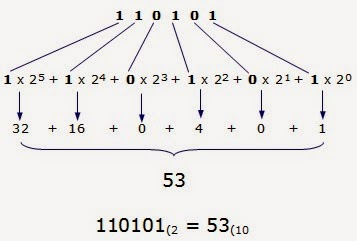
\includegraphics[width= 6cm]{imagen/binario-a-decimal-java.jpg}}
    \caption{Ejemplo Binario-Decimal}
    \label{fig}
\end{figure}

\subsubsection{Descripción del problema}

Dado un número binario de $n$ bits regresar su equivalente en decimal.\\

\subsubsection{Diseño de solución}

El proceso para convertir un número binario a decimal es un método diferente.

Consta de numerar los dígitos de derecha a izquierda comenzando desde cero, a cada número se le asigna la correspondiente potencia base 2 y al final se suman las potencias.\\

Lo primero que se debe realizar es ubicar una serie de potencias de dos que es la base del sistema binario, cuyo exponente va aumentando a medida que cambiamos la posición de derecha a izquierda, después se multiplica cada dígito del número binario por el resultado de la potencia, después se deben sumar los resultados para poder encontrar el número decimal.\\

\subsubsection{Desarrollo de la solución del problema}

\begin{enumerate}
    \item Se diseño un diagrama de flujo para poder realizar un programa en JAVA en el cual pide ingresar un número binario.
    \begin{javaCode}
     //ENTRADA
     System.out.println("Ingresa un numero binario");
            String numeroBin = in.nextLine();
            int longitud = numeroBin.length();
            int numeroDecimal = 0;
    \end{javaCode}
    \item A base de una codificación te mostrará como resultado el número decimal correspondiente al número binario ingresado.
     \begin{javaCode}
     //PROCESO
     for (int i = 0; i < longitud; i++) {
                
                char digito = numeroBin.charAt(i);
                
                //verificacion si es 0 o 1
                if (digito == '0') {
                    numeroDecimal *= 2;
                } else if(digito == '1') {
                    numeroDecimal = (numeroDecimal * 2) + 1;
                } else {
                    System.out.println("El numero binario ingresado no es valido");
                    return;
                }
            }
            
     \end{javaCode}
    \item Y al final se mirará reflejado el número decimal correspondiente al número binario solicitado.
    \begin{javaCode}
    //SALIDA
        System.out.println("El numero decimal equivalente es " + numeroDecimal);
    \end{javaCode}
 \end{enumerate}
\subsubsection{Depuración y pruebas}
A continuación en la siguiente tabla 5 se presentan los resultados de la prueba de compilación del código.

\begin{table}[!ht]
\label{T:equipos}
\begin{center}
\begin{tabular}{| c | c | c | c | c | c |}
\hline
\textbf{Número de corrida} & \textbf{Número binario} & \textbf{Número decimal}\\
\hline
1 & 10101 & 21 \\
2 & 1110001 & 113 \\
3 & 101010111 & 343 \\
\hline
\end{tabular}
\caption{Tabla de corridas.}
\end{center}
\end{table}\\


